如图2-5和2-6所示,可以在程序中构造多个队列。可以将这些队列绑定到单个设备上(队列的工作汇集到单个设备上),绑定到多个设备上,或者绑定到这些设备的组合上。以GPU绑定队列和FPGA绑定队列为例,如图2-13所示。对应的映射如图2-14所示。\par

\hspace*{\fill} \par %插入空行
图2-13 创建GPU和FPGA设备的队列
\begin{lstlisting}[caption={}]
#include <CL/sycl.hpp>
#include <CL/sycl/INTEL/fpga_extensions.hpp> // For fpga_selector
#include <iostream>
using namespace sycl;

int main() {
	queue my_gpu_queue( gpu_selector{} );
	queue my_fpga_queue( INTEL::fpga_selector{} );
	
	std::cout << "Selected device 1: " <<
		my_gpu_queue.get_device().get_info<info::device::name>() << "\n";
		
	std::cout << "Selected device 2: " <<
		my_fpga_queue.get_device().get_info<info::device::name>() << "\n";
	
	return 0;
}

//Possible Output:
//Selected device 1: Intel(R) Gen9 HD Graphics NEO
//Selected device 2: pac_a10 : PAC Arria 10 Platform
\end{lstlisting}

\hspace*{\fill} \par %插入空行
图2-14 GPU+FPGA设备选择器示例:一个队列绑定GPU,另一个队列绑定FPGA
\begin{center}
	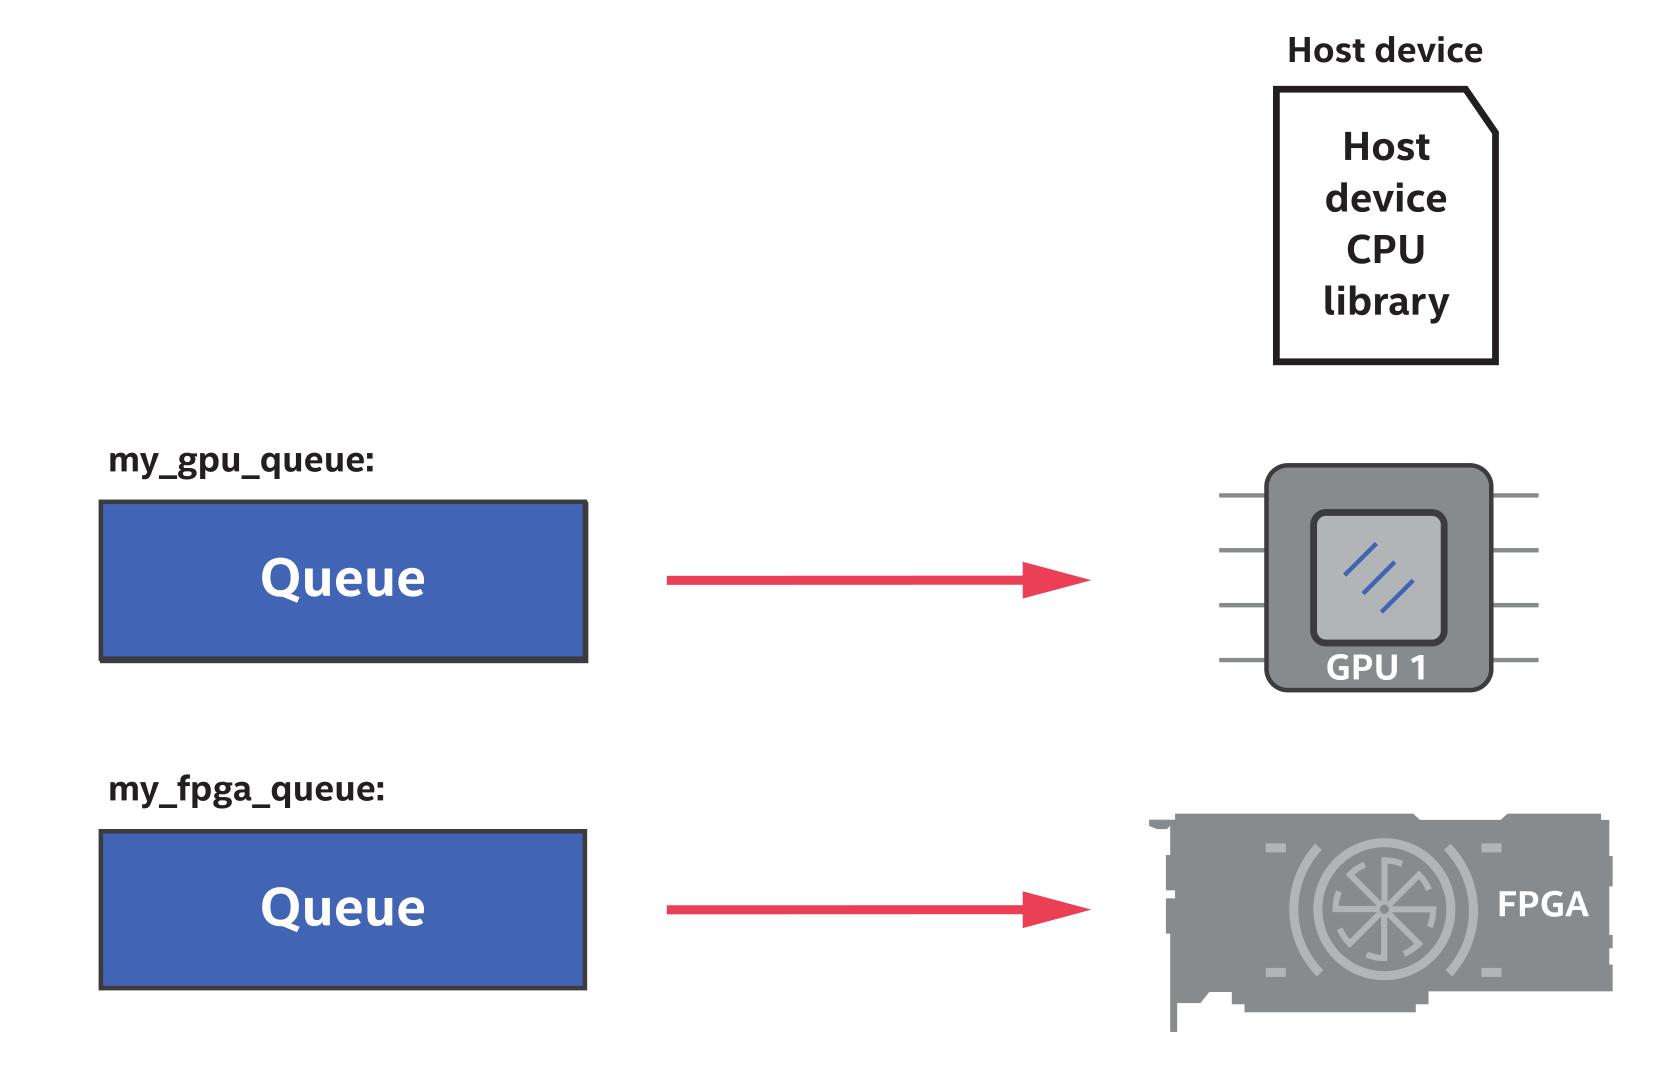
\includegraphics[width=0.8\textwidth]{content/chapter-2/images/8}
\end{center}












